%----------------------------------------------------------------------------------------
%	Capítulo 6
%----------------------------------------------------------------------------------------

\pagestyle{myportland}
\doublespacing
%\pagenumbering{arabic}
\chapter[\quad\quad\quad\quad ----- Pruebas y resultados]{\\ Pruebas y resultados}
\thispagestyle{myportland}

Este capítulo está enfocado en mostrar simulaciones o pruebas obtenidas en los algoritmos o mecanismos empleados en el sistema. Además desarrolla de manera técnica los resultados con la finalidad de ser comparables con resultados de otros autores de otras máquinas.






%% NUEVA SECCIÓN X.X
\section{Algoritmos de clasificación y conteo de truchas}

Los algoritmos seleccionados para realizar las pruebas son YOLOv3 y YOLOv4\footnote{Se puede probar las demos listadas en la sección \ref{ssec:repositorio de codigo fuente}.}. Las bases de datos empleadas en las pruebas para entrenar los algoritmos son la FISH9002 y FISH9003 de elaboración propia que contienen 723 y 2400 imágenes respectivamente. Sin embargo, se muestra únicamente resultados de la base de datos de imágenes FISH9003 ya que es esperable que brinde mejores resultados.

Con la versión 3 de esta arquitectura que sigue bajo desarrollo actualmente para mejorar el rendimiento. Las inferencias permiten detectar objetos para los cuales la red es entrenada mediante una gran cantidad de imágenes que contienen el objeto de interés. Para el procesamiento básicamente se realiza un redimensionamiento de la imagen antes de procesarla, luego diferentes arquitecturas de redes neuronales dentro de la arquitectura logran detectar el objeto. Luego de detectado el objeto se procede a segmentarlo mediante técnicas de enmascarado de objetos. Finalmente cada objeto detectado en la imagen es contabilizado dentro del programa. En la Figura \ref{fig:pruebas algoritmo} se muestra en el lado izquierdo la imagen que se ingresa al algoritmo y a la derecha el pez segmentado para ser contabilizado.

\begin{myfigure}[H]
	\footnotesize\centering
	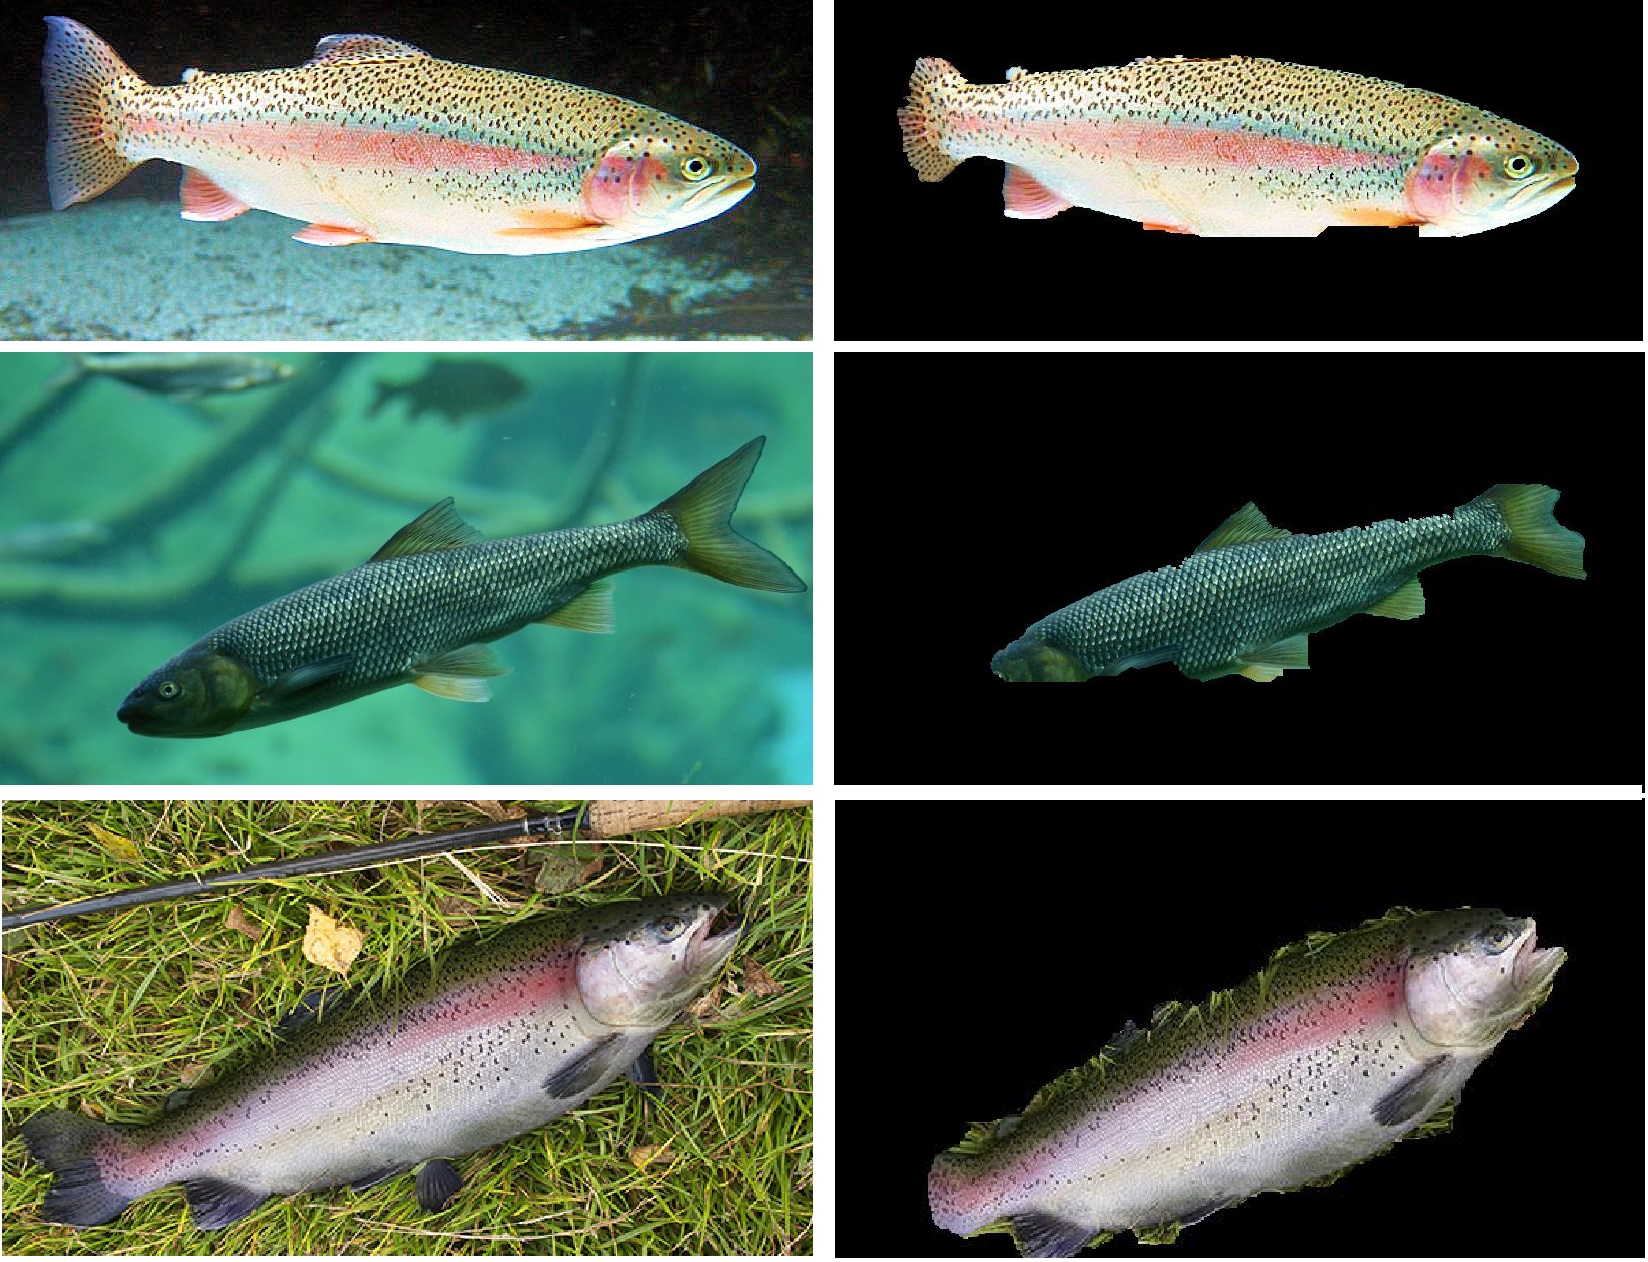
\includegraphics[width=1\textwidth]{chapter6/pruebas algoritmo.png}
	\caption{Inferencia de detección y conteo de truchas.}
	\begin{myflushcenter}
		Fuente: Elaboración propia.
	\end{myflushcenter}
	\label{fig:pruebas algoritmo}
\end{myfigure}

En el caso de la clasificación el sistema debe ser calibrado acorde al entorno, por lo que su etapa de desarrollo luego de la detección se da en la etapa de prototipado y producción. Sin embargo, el conteo es realizado sin ningún problema.





% NUEVA SECCIÓN X.X.X
\subsection{Definición de criterios de clasificación}

\footnote{Los términos técnicos usados son citados de \cite{Everingham2010}.}


\begin{myfigure}[H]
	\footnotesize\centering
	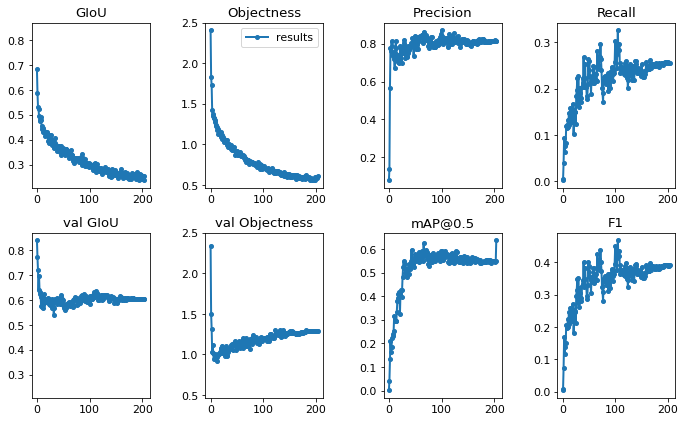
\includegraphics[width=1\textwidth]{chapter6/resultados yolo 3.png}
	\caption{Resultados del entrenamiento de YOLOv3.}
	\begin{myflushcenter}
		Fuente: Elaboración propia.
	\end{myflushcenter}
	\label{fig:resultados yolo 3}
\end{myfigure}



% NUEVA SECCIÓN X.X.X
\subsection{Resultados del entrenamiento de los algoritmos}

\textcolor{blue}{[BORRADOR] Lorem ipsum dolor sit amet, consectetur adipiscing elit, sed do eiusmod tempor incididunt ut labore et dolore magna aliqua. Lacus sed turpis tincidunt id aliquet. Nunc aliquet bibendum enim facilisis gravida neque convallis a. Ut tellus elementum sagittis vitae et leo duis ut diam. Dolor sit amet consectetur adipiscing elit ut aliquam purus sit. Dolor sed viverra ipsum nunc aliquet bibendum. Euismod in pellentesque massa placerat. Et malesuada fames ac turpis egestas sed tempus urna. Euismod elementum nisi quis eleifend quam adipiscing vitae proin. Ornare suspendisse sed nisi lacus sed. Mollis aliquam ut porttitor leo a diam. Varius morbi enim nunc faucibus. Sit amet purus gravida quis blandit turpis cursus in hac. [/BORRADOR]} 

% NUEVA SECCIÓN X.X.X
\subsection{Análisis de tiempo de ejecución del algoritmo}

\textcolor{blue}{[BORRADOR] Lorem ipsum dolor sit amet, consectetur adipiscing elit, sed do eiusmod tempor incididunt ut labore et dolore magna aliqua. Lacus sed turpis tincidunt id aliquet. Nunc aliquet bibendum enim facilisis gravida neque convallis a. Ut tellus elementum sagittis vitae et leo duis ut diam. Dolor sit amet consectetur adipiscing elit ut aliquam purus sit. Dolor sed viverra ipsum nunc aliquet bibendum. Euismod in pellentesque massa placerat. Et malesuada fames ac turpis egestas sed tempus urna. Euismod elementum nisi quis eleifend quam adipiscing vitae proin. Ornare suspendisse sed nisi lacus sed. Mollis aliquam ut porttitor leo a diam. Varius morbi enim nunc faucibus. Sit amet purus gravida quis blandit turpis cursus in hac. [/BORRADOR]} 

% NUEVA SECCIÓN X.X.X
\subsection{Errores detectados en la simulación de conteo de truchas}

\textcolor{blue}{[BORRADOR] Lorem ipsum dolor sit amet, consectetur adipiscing elit, sed do eiusmod tempor incididunt ut labore et dolore magna aliqua. Lacus sed turpis tincidunt id aliquet. Nunc aliquet bibendum enim facilisis gravida neque convallis a. Ut tellus elementum sagittis vitae et leo duis ut diam. Dolor sit amet consectetur adipiscing elit ut aliquam purus sit. Dolor sed viverra ipsum nunc aliquet bibendum. Euismod in pellentesque massa placerat. Et malesuada fames ac turpis egestas sed tempus urna. Euismod elementum nisi quis eleifend quam adipiscing vitae proin. Ornare suspendisse sed nisi lacus sed. Mollis aliquam ut porttitor leo a diam. Varius morbi enim nunc faucibus. Sit amet purus gravida quis blandit turpis cursus in hac. [/BORRADOR]} 

%\textcolor{blue}{[BORRADOR] Lorem ipsum dolor sit amet, consectetur adipiscing elit, sed do eiusmod tempor incididunt ut labore et dolore magna aliqua. Lacus sed turpis tincidunt id aliquet. Nunc aliquet bibendum enim facilisis gravida neque convallis a. Ut tellus elementum sagittis vitae et leo duis ut diam. Dolor sit amet consectetur adipiscing elit ut aliquam purus sit. Dolor sed viverra ipsum nunc aliquet bibendum. Euismod in pellentesque massa placerat. Et malesuada fames ac turpis egestas sed tempus urna. Euismod elementum nisi quis eleifend quam adipiscing vitae proin. Ornare suspendisse sed nisi lacus sed. Mollis aliquam ut porttitor leo a diam. Varius morbi enim nunc faucibus. Sit amet purus gravida quis blandit turpis cursus in hac. [/BORRADOR]} 


%% NUEVA SECCIÓN X.X
\section{Simulación estructural}

Las simulaciones estructurales se realizan dentro de softwares que permiten simular fuerzas, momentos y esfuerzos a los que se estima estará sometido los componentes mecánicos del sistema.

%% NUEVA SECCIÓN X.X.X
\subsection{Armadura}

La armadura de soporte hecha de perfiles cuadrados de acero inoxidable con norma ISO 316 tiene un factor de seguridad (F.S.) de sometido a las fuerzas presentes del sistema. En La Figura \ref{fig:simulacion armadura} se muestra un mapa de calor que muestra el factor de seguridad según la zona de la armadura. Como se muestra en la Figura  \ref{fig:simulacion armadura} el factor mínimo de seguridad es 15, por lo que se garantiza la integridad de la armadura sometida a las fuerzas y cargas esperadas.

\begin{myfigure}[H]
	\footnotesize\centering
	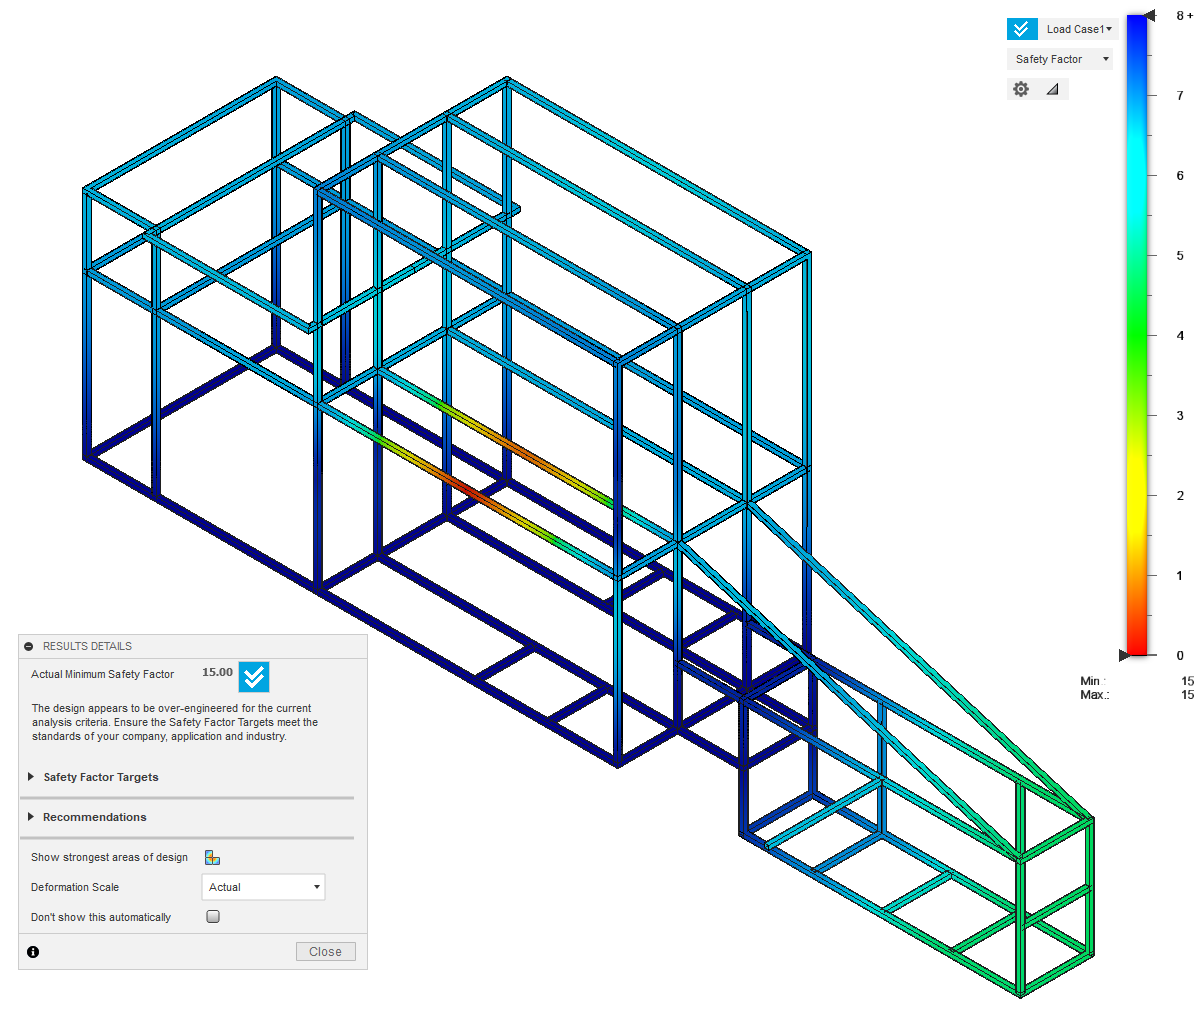
\includegraphics[width=1\textwidth]{chapter6/simulacion armadura.png}
	\caption{Cálculo de factor de seguridad de armadura en operación.}
	\begin{myflushcenter}
		Fuente: Elaboración propia.
	\end{myflushcenter}
	\label{fig:simulacion armadura}
\end{myfigure}


%% NUEVA SECCIÓN X.X.X
\subsection{Plataforma flotante}

Un componente clave a pesar de no estar dentro del diseño directo del sistema es la plataforma sobre la cual el sistema se apoya para ser estable en medio de un lago o laguna. La plataforma flotante fue diseñada y simulada bajo cargas de hasta 300 kilos repartidas en una área que ocupa el sistema que se propone. En la Figura \ref{fig:simulacion plataforma} se muestra que el factor de seguridad del sistema es de 15 lo cual nos indica que la plataforma soportará la carga sin problemas y no es riesgo para su flotabilidad.

\begin{myfigure}[H]
	\footnotesize\centering
	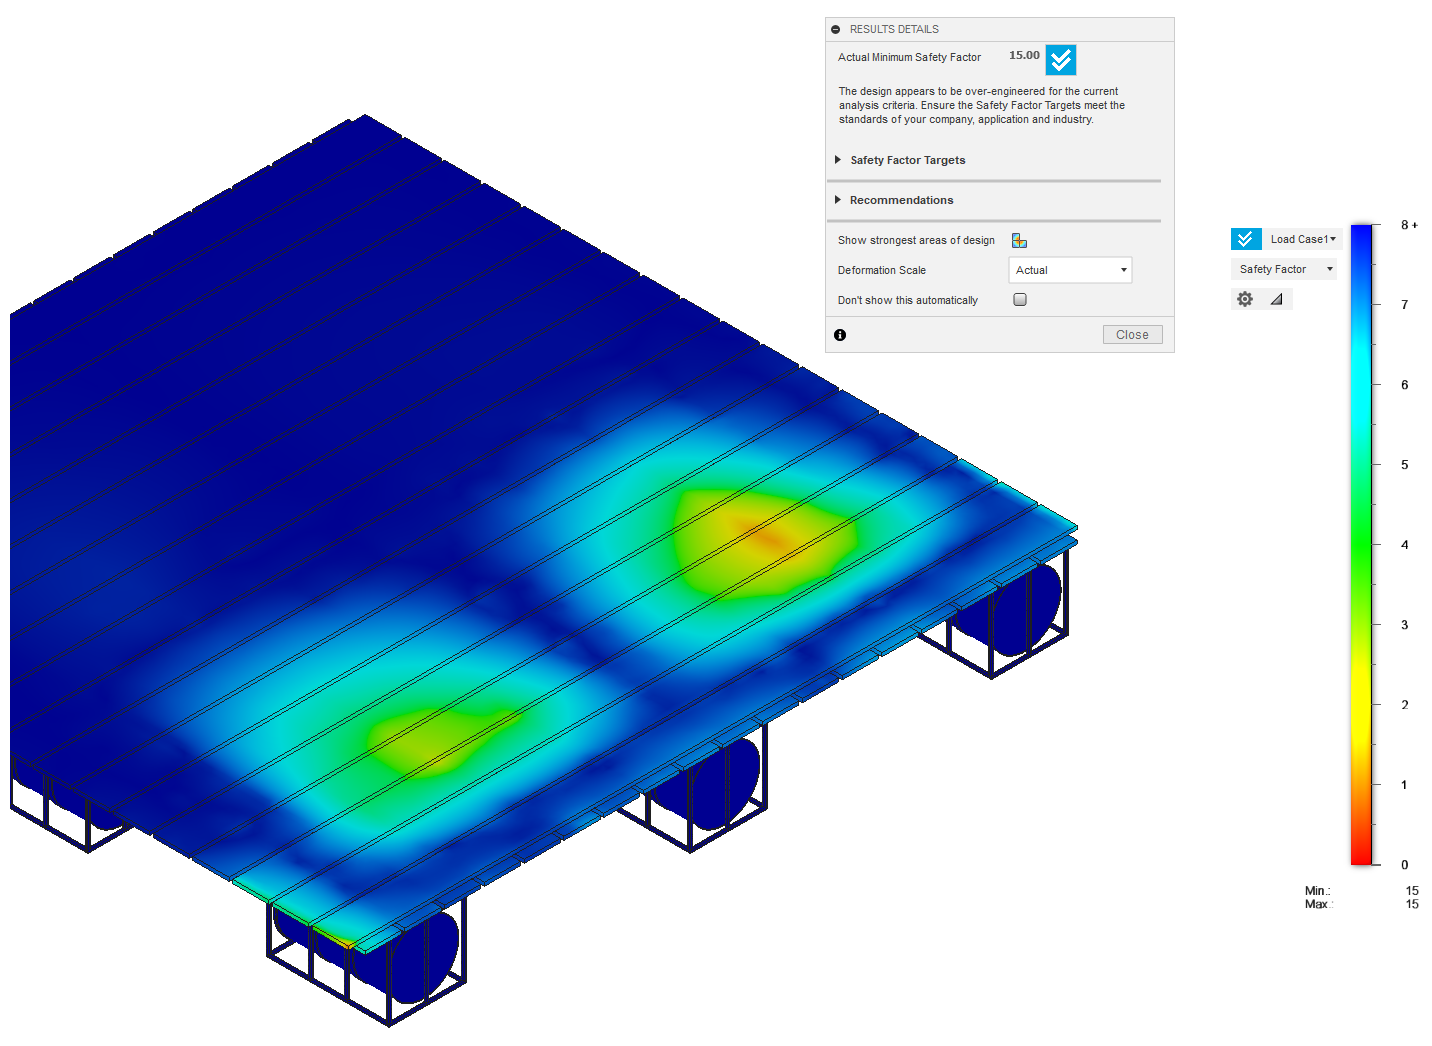
\includegraphics[width=1\textwidth]{chapter6/simulacion plataforma.png}
	\caption{Cálculo de factor de seguridad en la plataforma flotante de 5x5 m.}
	\begin{myflushcenter}
		Fuente: Elaboración propia.
	\end{myflushcenter}
	\label{fig:simulacion plataforma}
\end{myfigure}


%% NUEVA SECCIÓN X.X.X
\subsection{Distribuidora de truchas}

La distribuidora de truchas se elabora principalmente con procesos de plegado de metales, en este caso acero inoxidable AISI 316 y una placa de PMMA. La distribuidora no está sujeta a tensiones, compresiones o esfuerzos considerables, la única carga que posee es la de la trucha en tránsito. Por lo que se estudia la carga de la trucha dentro de sus compartimentos. En la Figura \ref{fig:simulacion distribuidora} se muestra un mapa de calor que muestra el factor de seguridad según la zona de la armadura.

\begin{myfigure}[H]
	\footnotesize\centering
	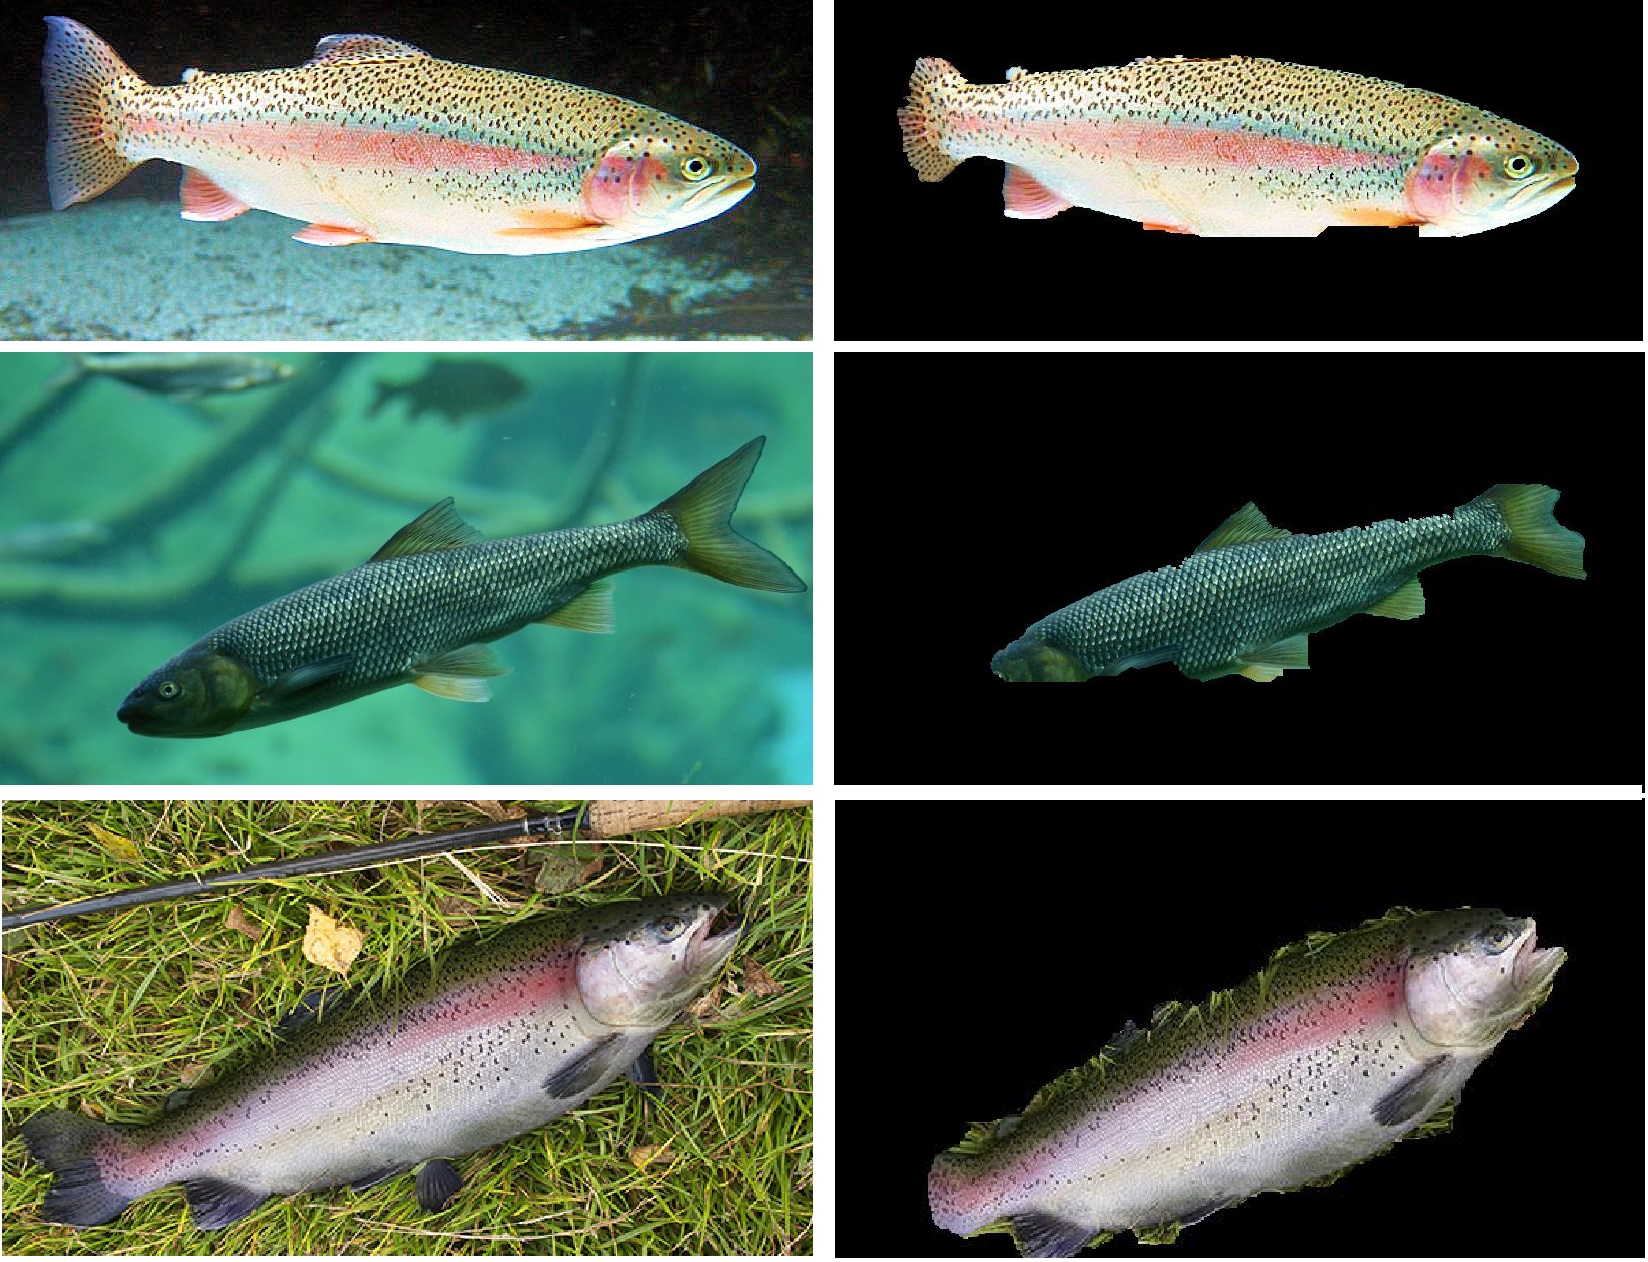
\includegraphics[width=1\textwidth]{chapter6/simulacion distribuidora.png}
	\caption{Cálculo de factor de seguridad en la distribuidora de truchas.}
	\begin{myflushcenter}
		Fuente: Elaboración propia.
	\end{myflushcenter}
	\label{fig:simulacion distribuidora}
\end{myfigure}



